\chapter{Identification du Sens du Résultat par Classification}
\label{sec:sensresultat}

\section{Objectif et Motivation}
\label{sec:sensresultat:motivation}
Dans ce chapitre, il est question d'extraire le sens du résultat d'une demande connaissant sa catégorie. Nous modélisons la tâche comme une classification binaire où un algorithme est entraîné à déterminer si la demande a été rejetée (sens = rejette) ou acceptée (sens = accepte). Cette modélisation est possible en s'appuyant sur les deux postulats suivants:

\begin{postulat}
Pour toute catégorie de demande $C$, on ne considère que les décisions dans lesquelles n'apparaît qu'une seule demande de catégorie $C$.
\end{postulat} 
Ce postulat est légitime car les statistiques sur les données labellisées de la Figure \ref{stat-alldata-dmd} montre bien que pour la majorité des catégories, peu de décisions contiennent plus d'une demande. On remarque néanmoins l'exception de la catégorie STYX (dommage-intérêt sur l'article 700 CPC), où dans la majorité des documents, on a plutôt 2 demandes. Cette exception peut se justifier par le fait que chaque partie fait généralement ce type de demande car elle porte sur le remboursement de frais de justice. Ce postulat présente cependant un inconvénient dû au fait que la majorité des demandes se trouvent dans des décisions à plus d'une demande. Il est donc possible de manquer un grand nombre de demandes. %On pourrait peut-être porter la classification à un modèle multi-label qui déterminera plusieurs sens à partir d'un seul document. Par exemple <SENS1, SENS2, SENS3> avec des valeurs prédéfinies sur les SENS 2 et 3 par exemple NO-DMD pour indiquer que la décision ne comprend pas de seconde ou de troisième demande.

\begin{postulat}
Le sens du résultat est binaire: accepte ou rejette.
\end{postulat} 
Ce postulat est justifié car le sens d'un résultat est pratiquement toujours une de ces deux valeurs (Figure \ref{stat-sensrst}). Les autres sens étant très rares, nous ne les considérons pas.

\begin{figure}
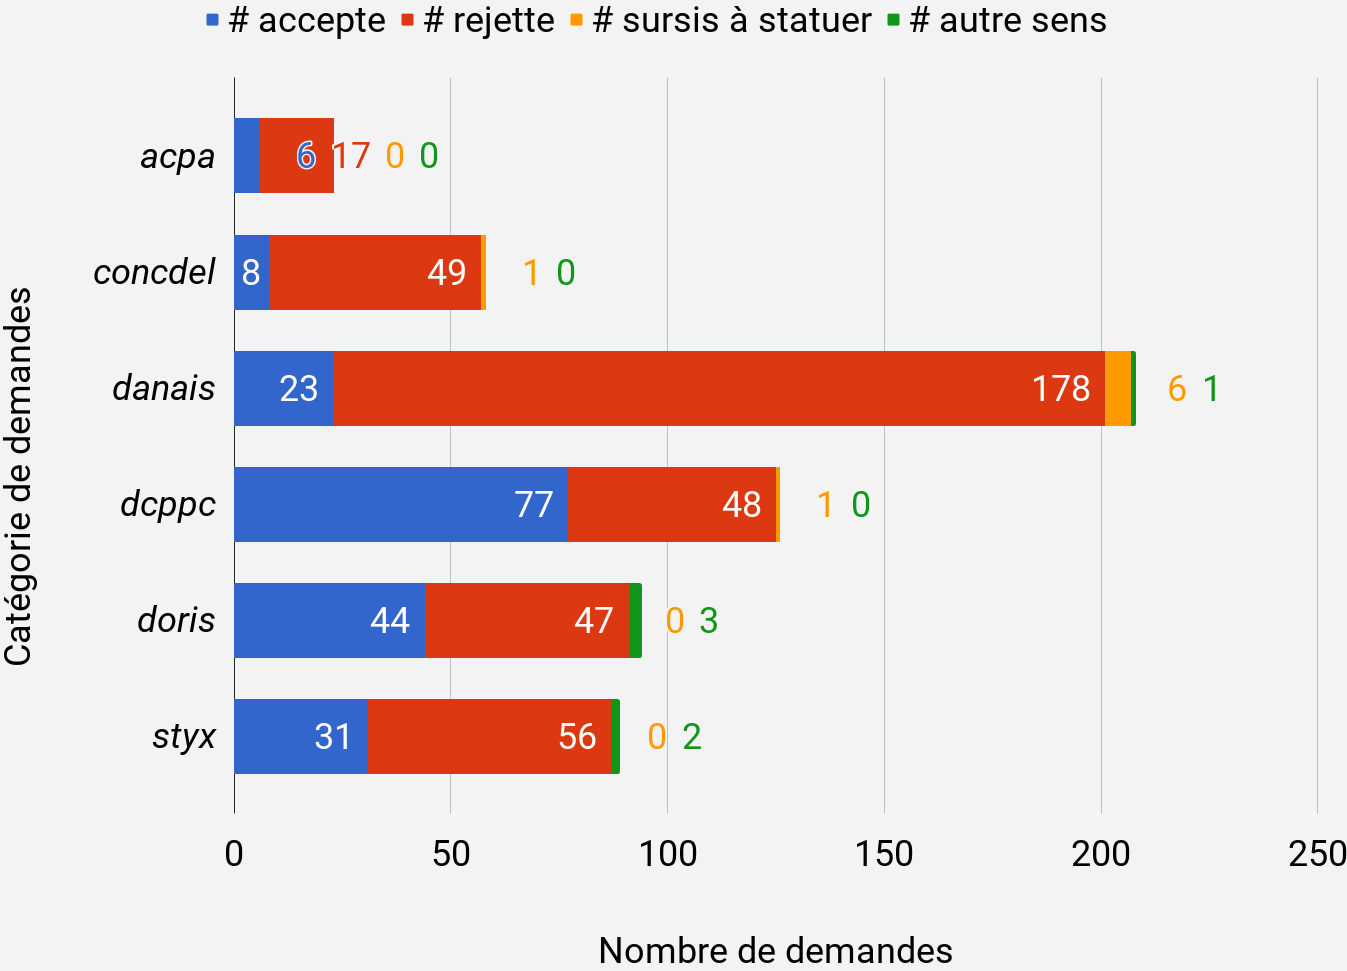
\includegraphics[width=\textwidth]{chartDistrSens.png}
\caption{Répartition des sens de résultat dans les données annotées.}\label{stat-sensrst}
\end{figure}
\section{Formulation du Problème}
\label{sec:sensresultat:probleme}

Cette étude porte sur l'analyse de l'impact de différents aspects techniques généralement appliqués dans le cadre de la classification de texte:
La représentation de texte (généralement vectorielle) faisant intervenir les notions de BagOfWord, TFIDF, poids global, poids local, matrice document-terme
La transformation de dimension a pour but de projeter le vecteur représentant un document dans un nouvel espace où généralement la distinction des classes est plus facile. Ceci est généralement effectuée en déterminant des composantes discriminantes à partir de la base d'entraînement: sélection de caractéristique, réduction matricielle, représentation vectorielle “sémantique” des documents (LatentDA, LSA, word embedding, ...)

 Cette analyse permettra de savoir s'il existe une certaine configuration permettant de déterminer le sens du résultat à une demande sans nécessairement l'avoir identifiée précisément dans le document. 


\section{Synthèse bibliographique: Classification de Texte}
\label{sec:sensresultat:biblio_classif}

La classification de texte permet d'organiser des documents dans des groupes prédéfinis. Elle reçoit depuis longtemps beaucoup d'attentions. Deux choix techniques influencent principalement les performances: la représentation des textes et l'algorithme de classification. Parmi les meilleurs algorithmes de classification binaire, les méthodes les plus populaires sont le NBSVM et FastText dont les performances pour l'analyse de sentiment sont très bonnes. Le principe du NBSVM \citep{wang2012nbsvm} consiste à transformer les caractéristiques des textes, réduites à leur simple présence en réalisant leur produit élément à élément avec le vecteur poids du classifieurs bayésien multinomial (calculé avec le vecteur présence de caractéristique). Le nouveau vecteur issu de ce produit représente le texte en entrée d'un SVM classique.
  
  Quant à FastText \citep{grave2017fasttextcls}, il s'agit d'un modèle de réseau de neurones dont l'architecture est semblable à celle de la variante CBOW de la méthode de plongement sémantique Word2Vec dans laquelle le mot du milieu a été remplacé par le label de la classe du texte. La classification est opérée par la fonction softmax $f(z) = \left[ \frac{e^{z_j}}{\sum\limits_{k=1}^K e^{z_k}} \right]_{\forall j \in \lbrace 1, ..., K \rbrace} $ et l'entraînement consiste à minimiser la fonction objectif $-\frac{1}{N}y_n \cdot \sum\limits_{n=1}^N y_n \cdot \log{f(B\cdot A\cdot x_n)}$ qui estime la distribution de probabilité des classes.

Le fonctionnement de ces deux méthodes intègrent leur propre représentation, contrairement aux algorithmes traitant des vecteurs comme le SVM. Il existe un très grand nombre de schémas de représentations vectorielles des documents


\section{Méthode: Extensions de la Regression PLS}
\label{sec:sensresultat:pls}
\textcolor{red}{Justification: Pourquoi le PLS?:}
https://link.springer.com/content/pdf/10.1007\%2FBF02174528.pdf, 
https://www.stat4decision.com/fr/regression-pls/
La regression PLS est une méthode de regression avec laquelle l'on tente d'expliquer une ou plusieurs variables Y (dite dépendantes) par des variables $X=x_1,x_2,...,x_p$ (dites explicatives). Elle consiste principalement de transformer les variables explicatives en un nombre réduit de composantes principales orthogonales $t_1, t_2, ..., t_h$. Les composantes $t_h$ sont construites étapes par étapes en applicant l'algorithme du PLS de façon récurrente sur les données mal prédites (résidus). Malgré ses quelques faiblesses comme celles liées au choix du nombre de composantes, à la complexité des sorties et la linéarité du modèle, le PLS présente quelques forces qui ont notamment de l'intérêt dans notre cas de figure. Par exemple, le PLS est gère assez bien la forte dispropotion entre le nombre de variables explicatives et le nombre d'observations, lorsque ce dernier est faible comme on peut l'observer dans nos données. Nous avons aussi la prise en compte de la multicolinéarité qui peut exister entre les variables explicatives, notamment quand celles-ci sont associées aux mots/termes souvent cooccurrents de nos documents.

Il est intéressant de noter la floraison d'extensions proposées pour répondre aux différentes limites du PLS. Notamment, nous pouvons citer la "\textit{sparse}" PLS introduit pour palier à la "\textit{sparsité}" et la colinéarité des variables explicatives [?], la PLS non-linéaire proposée pour les cas de données non-linéairement séparables [?], ou encore la PLS discriminante combinant la régression PLS et l'analyse discriminante [?]. Nos nous sommes intéressés à deux extensions particulières: la régression Gini-PLS dont l'intérêt est de réduire la sensibilités à la différence d'échelle de valeurs entre les variables, et la regression logistique PLS (Logit-PLS) combinant la regression logistique et la PLS.
\subsection{Gini-PLS}
\subsection{Logit-PLS}
\subsection{Logit-Gini-PLS}

\section{Expérimentations et interprétation des résultats}
\label{sec:sensresultat:experimentations}

\subsection{Données}
\label{subsec:sensresultat:xp:data}

\begin{figure}
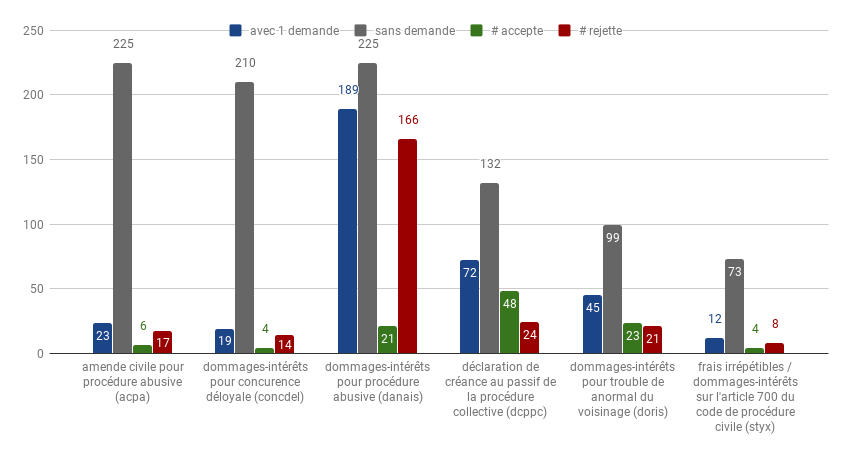
\includegraphics[width=\textwidth]{chartDataset1dmd.png}
\caption{Répartition des documents à une demande de la catégorie considérée.}\label{stat-1dmd}
\end{figure}

\section{Conclusion}
\label{sec:sensresultat:conclusion}